%----------------------------------------------------------------------------------------
%	PACKAGES AND THEMES
%----------------------------------------------------------------------------------------
\documentclass[aspectratio=169,xcolor=dvipsnames,handout]{beamer}
\usetheme{Darmstadt}
\usecolortheme{seahorse}

\usepackage[hangul]{kotex}

\usepackage{hyperref}
\usepackage{graphicx} % Allows including images
\usepackage{booktabs, multicol, multirow} % Allows the use of \toprule, \midrule and \bottomrule in tables
\setbeamercovered{transparent}
%----------------------------------------------------------------------------------------
%	TITLE PAGE
%----------------------------------------------------------------------------------------

\title[소득분배이론과 정책]{소득분배이론} % The short title appears at the bottom of every slide, the full title is only on the title page
\subtitle{경제정의와 불평등}

\author[오성재]{오성재}

\institute[HNU] % Your institution as it will appear on the bottom of every slide, may be shorthand to save space
{
    한남대학교 \\
    탈메이지 교양학부 \\
}
\date{\today} % Date, can be changed to a custom date


%----------------------------------------------------------------------------------------
%	PRESENTATION SLIDES
%----------------------------------------------------------------------------------------

\begin{document}

\begin{frame}
    % Print the title page as the first slide
    \titlepage
\end{frame}

\begin{frame}{목차}
    \tableofcontents
\end{frame}
%------------------------------------------------
%------------------------------------------------
\section{분배적 정의 이론}
%------------------------------------------------

\begin{frame}[<+->]
\frametitle{평등주의적 정의관}
    \begin{itemize}
        \item 모든 사람이 똑같은 도덕적 가치를 갖고 이 세상에 태어났다.
        \item 모두가 동일한 몫을 가져야 한다는 의미는 아님.
        \item 분배과정에서 개인의 권리, 자유 침해.
        \item 평등의 대상 : 최소한의 생활수준(minimum standard of living), 동등한 기회(equal opportunity).
    \end{itemize}
\end{frame}
%------------------------------------------------

\begin{frame}[<+->]
\frametitle{자유론적 정의관}
    \begin{itemize}
        \item 모든 사람이 {\bf 정당하게 가질 권리}가 있는 것들만을 소유하는 분배의 상태가 정의로운 것.
        \item 노직(R. Nozick) : 개인의 권리는 어떤 경우에도 침해될 수 없으며, 어느 누구도 사회 전체를 위한다는 미명 아래 다를 사람을 이용할 권리를 갖지 못한다.
        \item {\bf 정당한 권리의 원칙(entitlement principles)} : 소유의 과정에서 정당함, 결과의 정의보다 절차상의 정의를 중요.
        \item 결과로서 극단적 불평등도 절차적 정당성만 갖춰지면 정의로움.
    \end{itemize}
\end{frame}
%------------------------------------------------

\begin{frame}[<+->]
\frametitle{공리주의적 정의관}
    \begin{itemize}
        \item 벤담(J. Bentham) : 최대다수의 최대행복(the greatest happiness of the greatest number)
        \item 어떤 일의 옳고 그름은 그 일로 인해 사람들이 받는 영향을 좋고 나쁨에 달림.
        \item 평등한 결과에 호의적 : 모든 사람을 동일한 한 사람으로 간주.
        \item 불평등한 결과에도 호의적임.
    \end{itemize}
\end{frame}
%------------------------------------------------

\begin{frame}[<+->]
\frametitle{롤즈의 최소극대화 원칙}
    \begin{itemize}
        \item 평등주의적 자유주의자(egalitarian liberal)
        \item 원초적 상황(original position), 무지의 장막(veil of ignorance)
        \begin{block}{정의의 원칙}
            \begin{enumerate}
                \item 모든 사람은 다른 사람들의 자유와 양립할 수 있는 한, 가장 광범위하게 자유에 대해 동등한 권리를 가져야 한다.
                \item 사회적$\cdot$경제적 불평등은 다음의 두 조건을 모두 충족시킬 수 있을때만 그 정당성을 인정받을 수 있다.
                    \begin{enumerate}
                        \item 그 불평등이 모든 사람에게 이득이 될 것이라 합리적으로 기대할 수 있어야 한다.
                        \item 모든 사람에게 직위 및 직책(에 대한 접근)이 공정한 기회균등 하에 개방되어 있다.
                \end{enumerate}
            \end{enumerate}
        \end{block}
        \item 가정의 비현실성.        
    \end{itemize}
\end{frame}
%------------------------------------------------

%------------------------------------------------
\section{불평등 발생의 원인}
%------------------------------------------------

\begin{frame}[<+->]
    \begin{figure}
        \centering
        \includegraphics[width=.4\textwidth]{pic/ineqcircle.png}
        \caption{불평등 발생의 원인(이준구$\cdot$조명환 (2021), pp. 244)}
    \end{figure}
\end{frame}
%------------------------------------------------

\subsection{개인적 요인}

\begin{frame}[<+->]
\frametitle{원초적 단계}
    \begin{itemize}
        \item 유전적 요인 : 
        \begin{itemize}
            \item 외모, 신장, 유전병 등등.
        \end{itemize}
        \item 사회경제적환경(socio-economic status;SES) :
        \begin{itemize}
            \item 부모의 경제력.
            \item 부모의 학력.
            \item 부모의 직업.
        \end{itemize}
    \end{itemize}
\end{frame}
%------------------------------------------------

\begin{frame}[<+->]
\frametitle{중간적 단계}
    \begin{itemize}
        \item 비물질적 요인 : 
        \begin{itemize}
            \item 인지적 능력 : 지능(IQ) 등등.
            \item 비인지적 능력 : 정서, 심리, 육체적 능력 등등.
            \item 기타 개인적 특성.
        \end{itemize}
        \item 물질적 요인 : 
        \begin{itemize}
            \item 증여$\cdot$상속.
        \end{itemize}
        \item 교육수준과 부의 수준을 결정.
    \end{itemize}
\end{frame}
%------------------------------------------------

\begin{frame}[<+->]
\frametitle{경제적 지위의 격차}
    \begin{itemize}
        \item 직업적 지위 : 직업의 귀천은 없다?
        \item 소득 : 
        \begin{itemize}
            \item 근로소득.
            \item 비근로소득.
        \end{itemize}
    \end{itemize}
\end{frame}
%------------------------------------------------

\subsection{사회적 요인}

\begin{frame}[<+->]
\frametitle{체제 내적 요인}
    \begin{itemize}
        \item 재정제도 : 조세, 재분배 제도.
        \item 경제정책 : 개발계획, 사회안전망.
        \item 노동시장 : 산업구조조정.
        \item 가격변동 : 자산의 상대가격.
        \item 그 밖의 사회적 여건 : 차별, 부정부패.
    \end{itemize}
\end{frame}
%------------------------------------------------

\begin{frame}[<+->]
\frametitle{체제 자체의 성격}
    \begin{itemize}
        \item 순수자본주의 : 시장을 통한 효율적 분배만을 인정.
        \item 공산주의 : 부와 소득의 완전분배.
        \item 혼합경제체제 : 시장분배에 대한 정부의 재분배 용인.
    \end{itemize}
\end{frame}
%------------------------------------------------

\begin{frame}[<+->]
\frametitle{불평등 요인의 제거 가능성}
    \begin{itemize}
        \item 개인적 차원의 비물질적 경로로 인한 불평등의 제거는 현실적으로 어려움.
        \item 개인적 차원의 물질적 경로로 인한 불평등의 제거는 가능.
        \item 사회적 차원에서 발생하는 인한 불평등의 제거 역시 가능.
    \end{itemize}
\end{frame}
%------------------------------------------------

%------------------------------------------------
\section{재분배정책}
%------------------------------------------------

\begin{frame}[<+->]
\frametitle{재분배정책 반대논리}
    \begin{itemize}
        \item 윤리적 관점 :
        \begin{itemize}
            \item 자유론적 관점 : 자격이론.
            \item 불균등한 분배는 개인의 선택의 결과.
        \end{itemize}
        \item 효율성에 대한 부정적 영향 :
        \begin{itemize}
            \item 최고소득, 최저소득 계층의 근로의욕 저하.
        \end{itemize}
        \item 정치적 현실의 관점 : 
        \begin{itemize}
            \item 정부는 분배문제의 효율적 대안인가?
            \item 계층간 갈등 조장 : 수혜계층과 나머지 간의 갈등 유발.  
        \end{itemize}
    \end{itemize}
\end{frame}
%------------------------------------------------

\begin{frame}[<+->]
\frametitle{재분배정책 찬성논리}
    \begin{itemize}
        \item 윤리적 관점 : 
        \begin{itemize}
            \item 평등주의 : 평등분배만이 정의로운 분배.
            \item 공리주의 : 사회후생의 총합을 늘릴 수 있다면 재분배 정책은 옳음.
        \end{itemize}
        \item 공공재로서의 공평한 분배
        \begin{itemize}
            \item 더로우(L. Thurow, 1971): 재분배가 가져오는 사회적 이득은 공공재적 성격.
        \end{itemize}
        \item 사회보험으로서의 재분배
        \begin{itemize}
            \item 불의의 위기로 부터의 안전장치.
        \end{itemize}
        \item 정치적 관점
        \begin{itemize}
            \item 권력집중 방지 : 부를 차지하는 개인들은 권력 역시 차지하려고 함.
        \end{itemize}
    \end{itemize}
\end{frame}
%------------------------------------------------

\begin{frame}[<+->]
\frametitle{정부지출 : 전가의 문제}
    \begin{itemize}
        \item 정부지출에서 혜택의 전가(shifting)가 있을 경우 효과의 실제 귀착(actual incidence)은 의도와 다른 결과를 가져온다.
        \begin{exampleblock}{예시}
            \begin{itemize}
                \item 고등교육 지원이 불평등을 야기한다. 
                \begin{itemize}
                    \item 대학에 지원을 늘리면 대학을 진학하지 못한 개인들이 더 차별 받음.
                \end{itemize}
                \item 저소득 지역에 공공투자(지하철)는 거주민에게 해롭다.
                \begin{itemize}
                    \item 젠트리피케이션 현상의 발생.
                \end{itemize}
            \end{itemize}
        \end{exampleblock}
    \end{itemize}
\end{frame}
%------------------------------------------------

\begin{frame}[<+->]
\frametitle{정부지출 : 시장의 반응}
    \begin{itemize}
        \item 정부지출에서 혜택의 전가(shifting)는 해당 재화에 대한 시장의 수요와 공급에 의해서 결정되기도 한다.
            \begin{itemize}
                \item 수요(demand)곡선: 주어진 재화 또는 용역에 대하여 다른 조건들이 일정할때 제시된 가격에 대하여 시장참여자(소비자)들이 소비하기를 원하는 수량의 계획. 
                \item 공급(supply)곡선 : 주어진 재화 또는 용역에 대하여 다른 조건들이 일정할때 제시된 가격에 대하여 시장참여자(공급자)들이 공급하기를 원하는 수량의 계획. 
            \end{itemize}
        \item 정상재화의 경우 가격이 오를수록 시장의 수요량은 감소하고 공급량은 증가. 
        \item 가격 이외에 다양한 요건들이 수요와 공급에 영향(예 : 개인들의 소득, 기술발전 등등).
        \item 가격에 대하여 재화의 수요와 공급의 탄력성은 상이.
    \end{itemize}
\end{frame}

\begin{frame}
\frametitle{정부지출 : 시장의 반응(수요-공급 곡선)}
    \begin{columns}
        \begin{column}{.5\textwidth}<1->
            \begin{figure}
                \centering
                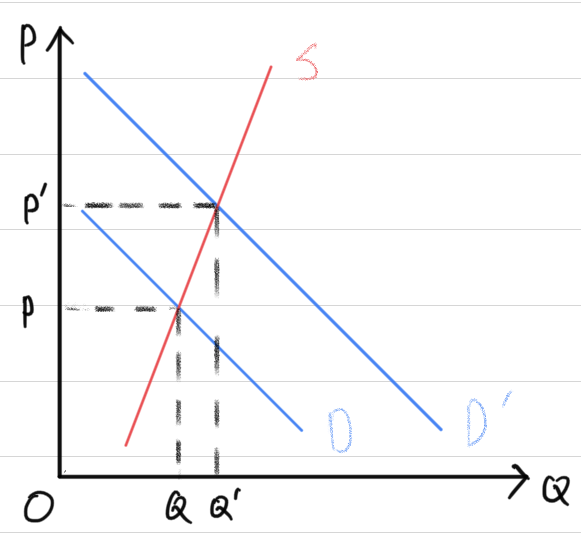
\includegraphics[width=.8\textwidth]{pic/helasup.png}
                \caption{비탄력적 공급}
            \end{figure}
        \end{column}
        \begin{column}{.5\textwidth}<2>
            \begin{figure}
                \centering
                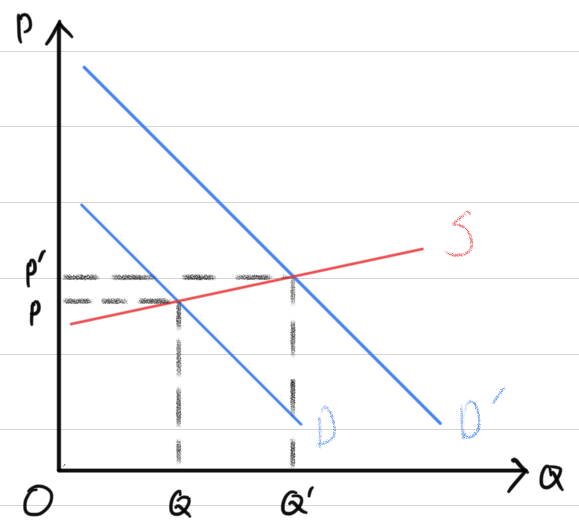
\includegraphics[width=.8\textwidth]{pic/lelasup.png}
                \caption{탄력적 공급}
            \end{figure}
        \end{column}
    \end{columns}
\end{frame}
%------------------------------------------------

\begin{frame}[<+->]
\frametitle{일반적 조세제도}
    \begin{itemize}
        \item 조세의 누진성(progressivity) : 납세자의 소득수준이 높아질수록 더 큰 비율의 세금을 납부.
        \item 조세제도의 특성에 따라 누진성이 변함 : 직접세(소득세) vs. 간접세(물품세).
        \item 높은 소득세가 반드시 높은 누진성을 동반하지 않음 : 공제제도, 유리지갑.
    \end{itemize}
\end{frame}
%------------------------------------------------

\begin{frame}[<+->]
\frametitle{부의 소득세제(Negative Income Tax)I}
    \begin{itemize}
        \item 개인의 소득이 일정 이하가 되면 음의 세울이 적용 됨. 
        \item 장점
        \begin{itemize}
            \item 권리 형식의 재분배 : 수혜자의 거부감이 적음.
            \item 행정적 편의성.
        \end{itemize} 
    \end{itemize}
\end{frame}
%------------------------------------------------

\begin{frame}
\frametitle{부의 소득세제II}
    \begin{columns}
        \begin{column}{.5\textwidth}<1->
            \begin{itemize}
                \item 시장소득 : $E$.
                \item 기초수당 : $m$.
                \item 한계세율 : $t$.
                \item 보조금 $S= max(0,m-tE)$
                \item 가처분소득 $Y = E + S$
            \end{itemize}
        \end{column}
        \begin{column}{.5\textwidth}<2>
            \begin{figure}
                \centering
                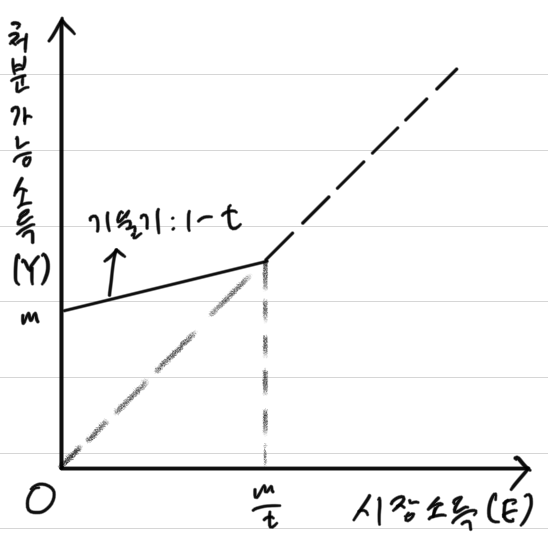
\includegraphics[width=.8\textwidth]{pic/nitax.png}
                \caption{부의 소득세제}
            \end{figure}
        \end{column}
    \end{columns}
\end{frame}
%------------------------------------------------

\begin{frame}[<+->]
\frametitle{부의 소득세제III}
    \begin{itemize}
        \item 단점
        \begin{itemize}
            \item 특수한 목적의 재분배 정책을 취할 수 없음.
            \item 재정적 부담.
            \item 경계에 있는 사람들의 근로의욕 저하.
            \item 장기적인 빈곤 탈피 효과에 의문.
        \end{itemize} 
    \end{itemize}
\end{frame}

%------------------------------------------------
\begin{frame}[<+->]
\frametitle{근로장려세제I(Earned Income Tax Credit;EITC)}
    \begin{itemize}
        \item 한국 2008년, 미국 1975년에 각각 시행.
        \item 개인의 소득이 일정 이하가 되면 음의 세울이 적용 됨. 
        \item 장점
        \begin{itemize}
            \item 공공부조 프로그램에 비해 근로의욕 저하가 적음.
        \end{itemize} 
        \item 개인의 근로시간 선택 문제 : 
        \begin{itemize}
            \item 개인은 취업을 여부 및 근로시간을 자유롭게 결정 할 수 있음.
            \item 개인은 24시간의 자유시간을 가지고 여가와 노동 중에 선택 가능.
            \item 개인은 여가와 노동이라는 재화에 대하여 일반적인 선호를 가짐.
        \end{itemize} 
    \end{itemize}
\end{frame}

\begin{frame}
\frametitle{근로장려세제II}
    \begin{columns}
        \begin{column}{.5\textwidth}<1->
            \begin{figure}
                \centering
                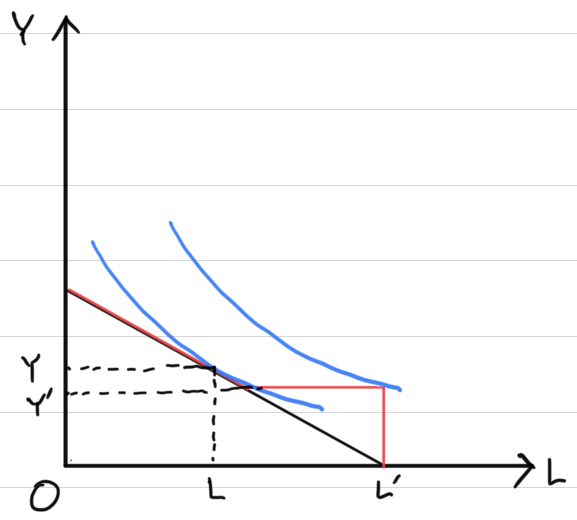
\includegraphics[width=.8\textwidth]{pic/pubsub.png}
                \caption{공공부조 제도}
            \end{figure}
        \end{column}
        \begin{column}{.5\textwidth}<2>
            \begin{figure}
                \centering
                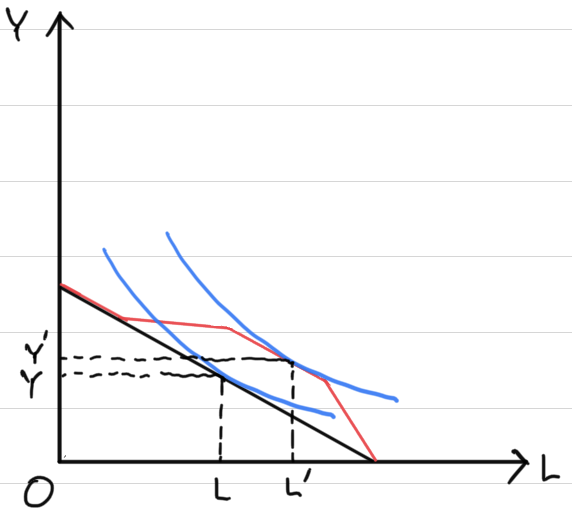
\includegraphics[width=.8\textwidth]{pic/eitc.png}
                \caption{부의 소득세제}
            \end{figure}
        \end{column}
    \end{columns}
\end{frame}
%------------------------------------------------

\end{document}
